\documentclass[12pt, a4paper, oneside]{ctexart}
\usepackage{amsmath, amsthm, amssymb, bm, color, framed, graphicx, hyperref, mathrsfs}

\title{\textbf{电介质习题}}
\author{韩岳成 524531910029}
\date{\today}
\linespread{1.5}
\definecolor{shadecolor}{RGB}{241, 241, 255}
\newcounter{problemname}
\newenvironment{problem}{\begin{shaded}\stepcounter{problemname}\par\noindent\textbf{题目\arabic{problemname}. }}{\end{shaded}\par}
\newenvironment{solution}{\par\noindent\textbf{解答. }}{\par}
\newenvironment{note}{\par\noindent\textbf{题目\arabic{problemname}的注记. }}{\par}

\begin{document}

\maketitle

\begin{problem}
    如图,一半径为R的介质球,试分别计算下列两种情况下电介质球表面上的极化面电荷密度和极化电荷的总和。已知极化强度

    (1)$\mathbf{P}= P_0$;

    (2)$\mathbf{P}= P_0 \frac{x}{R}$.

    \begin{center}
        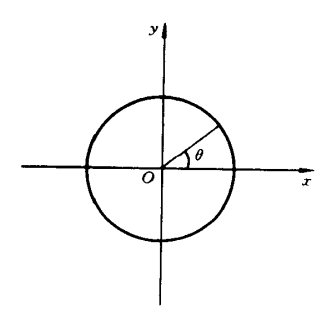
\includegraphics[width=0.3\textwidth]{HW1025-1.png}
    \end{center}
\end{problem}

\begin{solution}
    (1)由极化强度的定义,极化面电荷密度为
    \[\sigma' = \mathbf{P} \cdot \hat{n} = P_0 \cos \theta.\]
    总的极化电荷为
    \[q' = \int \sigma' dS = \int_0^{2\pi} \int_0^{\pi} P_0 \cos \theta R^2 \sin \theta d\theta d\phi = 0.\]

    (2)极化面电荷密度为
    \[\sigma' = \mathbf{P} \cdot \hat{n} = P_0 \frac{R \cos\theta}{R} \cos \theta = P_0 \cos^2 \theta.\]
    总的极化电荷为
    \[q' = \int \sigma' dS = \int_0^{2\pi} \int_0^{\pi} P_0  \cos^2 \theta R^2 \sin \theta d\theta d\phi = \frac{4\pi P_0 R^2}{3}.\]
    
\end{solution}

\begin{problem}
平行板电容器,板面积为 $100 cm^{2}$,带电量 $\pm 8.9×10^{-7} C$,在两板间充满电介质后,其场强为$ 1.4×10^{6} V/m$,试求

(1) 介质的相对介电常数 $\varepsilon_{r}$;

(2) 介质表面上的极化面电荷密度.
\end{problem}

\begin{solution}
    已知平行板电容器的电场强度为
    \[E = \frac{\sigma}{\varepsilon_0 \varepsilon_r},\]
    其中$\sigma = \frac{Q}{S}$为板上的电荷面密度。由此可得
    \[\varepsilon_r = \frac{Q}{\varepsilon_0 S E} = \frac{8.9 \times 10^{-7}}{8.85 \times 10^{-12} \times 100 \times 10^{-4} \times 1.4 \times 10^{6}} \approx 7.18.\]

    极化面电荷密度为
    \[\sigma' = P = \varepsilon_0(\varepsilon_r-1)E = 8.85 \times 10^{-12} \times (7.18-1) \times 1.4 \times 10^{6} \approx 7.66 \times 10^{-5} C/m^2.\]
\end{solution}

\begin{problem}
面积为 $S$ 的平行板电容器,两板间距为$d$,求

(1)插入厚度为$\frac d3$,相对介电常数为$\varepsilon_\mathrm{\tau}$的电介质,其电容变为原电容的多
少倍?

(2) 插入厚度为$\frac d3$的导体板,其电容又变为原电容的多少倍?
\end{problem}

\begin{solution}
(1) 假设插入的电介质的位置在电容器的中间,则可将新的电容器视为两个空气电容器与一个电介质电容器串联,电介质电容器的板间距为$\frac d3$,介电常数为$\varepsilon_\mathrm{\tau}$,另两个空气电容器的板间距为$\frac{d}3$,介电常数为$1$。则新的电容器的电容为
\[\frac 1C = \frac{1}{C_1} + \frac{1}{C_2} + \frac{1}{C_3} = \frac{d/3}{\varepsilon_0 \varepsilon_\mathrm{\tau} S} + 2 \times \frac{d/3}{\varepsilon_0 S} = \frac{d}{3 \varepsilon_0 S} \left(\frac 1{\varepsilon_\mathrm{\tau}} + 2\right).\]
因此新的电容为
\[C = \frac{3 \varepsilon_0 S}{d} \cdot \frac{\varepsilon_\mathrm{\tau}}{1 + 2 \varepsilon_\mathrm{\tau}}.\]
原电容为
\[C_0 = \frac{\varepsilon_0 S}{d}.\]
因此电容的变化倍数为
\[\frac{C}{C_0} = \frac{3 \varepsilon_\mathrm{\tau}}{1 + 2 \varepsilon_\mathrm{\tau}}.\]

(2) 插入导体板后,电容器的电容变为
\[C' = \frac{\varepsilon_0 S}{d - \frac{d}{3}} = \frac{3 \varepsilon_0 S}{2d}.\]
因此电容的变化倍数为
\[\frac{C'}{C_0} = \frac{3}{2}.\]
\end{solution}

\begin{problem}
在两个带等量异号电荷的平行金属板所产生的匀强电场内,充满均匀介质后,若已知自由电荷与极化电荷的面电荷密度分别为$\sigma_{_0}$与$\sigma^\prime$(绝对值),试求:

(1)电介质内的场强$E;$ 

(2) 相对介电常数$\varepsilon_{\mathrm{r}}.$
\end{problem}

\begin{solution}
(1) 由高斯定律可知,电介质内的场强为
\[E = \frac{\sigma_0 - \sigma'}{\varepsilon_0}.\]

(2) 由极化电荷密度与极化强度的关系可知
\[\sigma' = P \cdot \hat{n} = \varepsilon_0(\varepsilon_r - 1)E.\]
因此
\[\varepsilon_r = 1 + \frac{\sigma'}{\varepsilon_0 E} = \frac{\sigma_0}{\sigma_0 - \sigma'}.\]
\end{solution}

\begin{problem}
电学理论证明:一球形均匀电介质放在均匀外电场中会发生均匀极化.若已知此极化介质球的半径$R$,极化强度为$P.$试求极化电荷在球心处产生的场强$E^{\prime}$.
\end{problem}

\begin{solution}
考虑一个半径为 $R$ 的均匀极化球体,极化强度为 $\mathbf{P} = P \hat{\mathbf{z}}$。球面上的极化面电荷密度为:
$$\sigma' = \mathbf{P} \cdot \hat{\mathbf{n}} = P \cos \theta$$
其中 $\theta$ 是极角。
球心处的电场由所有极化面电荷贡献。面元 $dA$ 上的电荷为 $dq = \sigma' dA$,其在球心处产生的电场为:
$$
d\mathbf{E'} = \frac{1}{4\pi\epsilon_0} \frac{dq}{R^2} (-\hat{\mathbf{r}}) = -\frac{1}{4\pi\epsilon_0} \frac{\sigma' dA}{R^2} \hat{\mathbf{r}}$$
其中 $-\hat{\mathbf{r}}$ 表示从面元指向球心的方向。
球坐标下的面积元为 $dA = R^2 \sin \theta d\theta d\phi$,代入得:
$$d\mathbf{E'} = -\frac{1}{4\pi\epsilon_0} \sigma' \sin \theta d\theta d\phi \hat{\mathbf{r}}$$
总电场为:
$$
\mathbf{E'} = -\frac{1}{4\pi\epsilon_0} \oint \sigma' \hat{\mathbf{r}} \sin \theta d\theta d\phi$$
代入$\sigma^\prime=P\cos\theta:$

$$\mathbf{E}^{\prime}=-\frac P{4\pi\varepsilon_0}\int_0^{2\pi}\int_0^\pi\cos\theta\hat{\mathbf{r}}\sin\theta d\theta d\phi $$

将$\hat{\mathbf{r}}$用直角坐标分量表示:

$$\hat{\mathbf{r}}=\sin\theta\cos\phi\hat{\mathbf{x}}+\sin\theta\sin\phi\hat{\mathbf{y}}+\cos\theta\hat{\mathbf{z}}$$

代入积分:

$$\mathbf{E}^{\prime}=-\frac P{4\pi\varepsilon_0}\int_0^{2\pi}\int_0^\pi\cos\theta(\sin\theta\cos\phi\hat{\mathbf{x}}+\sin\theta\sin\phi\hat{\mathbf{y}}+\cos\theta\hat{\mathbf{z}})\sin\theta d\theta d\phi $$

分别计算三个分量:

x分量:

$$E_x^{\prime}=-\frac P{4\pi\varepsilon_0}\int_0^{2\pi}\cos\phi d\phi\int_0^\pi\cos\theta\sin^2\theta d\theta $$

其中$\int_0^{2\pi}\cos\phi d\phi=0$,故$E_x^\prime=0$

y分量:

$$E_y^{\prime}=-\frac P{4\pi\varepsilon_0}\int_0^{2\pi}\sin\phi d\phi\int_0^\pi\cos\theta\sin^2\theta d\theta $$

其中$\int_0^{2\pi}\sin\phi d\phi=0$,故$E_y^{\prime}=0$

z分量:

$$E_z^\prime=-\frac P{4\pi\varepsilon_0}\int_0^{2\pi}d\phi\int_0^\pi\cos^2\theta\sin\theta d\theta $$

计算积分:

$$\int_0^{2\pi}d\phi=2\pi,\quad\int_0^{\pi}\cos^2\theta\sin\theta d\theta=\frac23$$

所以:

$$E_z^{\prime}=-\frac P{4\pi\varepsilon_0}\cdot2\pi\cdot\frac23=-\frac P{3\varepsilon_0}$$

因此,极化电荷在球心处产生的电场为:

\[\mathbf{E}^{\prime}=-\frac P{3\varepsilon_0}\hat{\mathbf{z}}=-\frac{\mathbf{P}}{3\varepsilon_0}\]
\end{solution}

\begin{problem}
半径为 $R$ 的导体球,带电量为 $q$, 球外有一均匀介质的同心球壳,内外半径分别为 $r_{1}$ 和 $r_{2}$, 相对介电常数为 $\varepsilon_{r}$ . 求:

(1) 介质内、外的$ E$ 和$ D$;

(2) 介质内的极化强度 $P$ 和半径 $r_{2}$ 处表面上的极化面电荷密度 $\sigma'$.

\begin{center}
        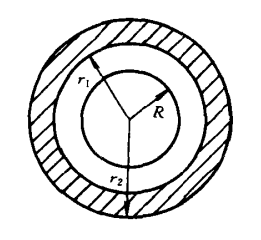
\includegraphics[width=0.3\textwidth]{HW1025-2.png}
    \end{center}
\end{problem}

\begin{solution}
由于系统具有严格的球对称性,电场与位移矢量均沿径向方向:

\[
\mathbf{E}(r)=E(r)\,\hat{\mathbf{r}},\qquad \mathbf{D}(r)=D(r)\,\hat{\mathbf{r}}.
\]

取半径为 $r$ 的高斯面,有
\[
\oint \mathbf{D}\cdot d\mathbf{S} = D(r)\cdot 4\pi r^2 = q,
\]
因此
\[
D(r) = \frac{q}{4\pi r^2}.
\]
介质内有
\[
\mathbf{D}=\varepsilon \mathbf{E}=\varepsilon_0\varepsilon_r \mathbf{E},
\]
故
\[
\mathbf{E}(r)=\frac{q}{4\pi\varepsilon_0\varepsilon_r r^2}\hat{\mathbf{r}},\qquad
\mathbf{D}(r)=\frac{q}{4\pi r^2}\hat{\mathbf{r}}\qquad (r_1<r<r_2).
\]

对于介质外部:
\[
\mathbf{E}(r)=\frac{q}{4\pi\varepsilon_0 r^2}\hat{\mathbf{r}},\qquad
\mathbf{D}(r)=\frac{q}{4\pi r^2}\hat{\mathbf{r}}\qquad (r>r_2).
\]

(2) 介质中极化强度为
\[
\mathbf{P} = \varepsilon_0(\varepsilon_r-1)\mathbf{E}.
\]
代入介质内电场得
\[
\mathbf{P}(r)=\frac{q(\varepsilon_r-1)}{4\pi\varepsilon_r r^2}\hat{\mathbf{r}}\qquad (r_1<r<r_2).
\]
极化表面电荷密度为
\[
\sigma' = \mathbf{P}\cdot \hat{\mathbf{n}}.
\]
在半径 $r_2$ 处,法向量 $\hat{\mathbf{n}}=\hat{\mathbf{r}}$,故
\[
\sigma'(r_2)=\frac{q(\varepsilon_r-1)}{4\pi\varepsilon_r r_2^2}.
\]

\end{solution}
\end{document}


\end{solution}
\end{document}
